\vspace{-.15in}\section{Research Plan and Methodology}
\label{sec:rep}\vspace{-.075in}

% \xxx strengthens the reliability of datacenter 
% computing with a holistic methodology.
This section first proposes \falcon 
(\S\ref{sec:protocol}), a fast consensus protocol, it then leverages \falcon to 
construct a scheduler (\S\ref{sec:scheduler}) and a VM (\S\ref{sec:vm}) for 
application availability. Finally, it describes 
research plan (\S\ref{sec:plan}).
% The first two objectives include preliminary results. 

\vspace{-.15in}\subsection{Objective 1: building fast distributed consensus via
RDMA}\label{sec:protocol}\vspace{-.075in}

This section presents \paxos performance problem (\S\ref{sec:latency-problem}) 
and a fast, RDMA-powered protocol (\S\ref{sec:falcon}).

\vspace{-.15in}
\subsubsection{Problem: consensus latency of existing \paxos 
protocols are slow and unscalable} 
\label{sec:latency-problem}\vspace{-.075in}

% P1: as mentioned in background, a key reason is thread interleavings, 
% so we need to reason about the general patterns we have. Or we say our 
% methodology is just like pattern matching.
% Traditional \paxos protocols incur high consensus latency because they go 
% through OS kernels and software TCP/IP layers. In this 
% section, \S\ref{sec:problem} analyzes this latency problem and its poor 
% scalability in detail, and then presents our new RDMA-based \paxos 
% protocol called \falcon (\S\ref{sec:falcon}).

% First, mainly introduce the problems in traditional protocols.
% Due to the strong fault-tolerance of \paxos, it is widely served in many 
% systems. For instance, Scatter~\cite{scatter:sosp11} runs 8$\sim$12 replicas in 
% each \paxos group to order client requests, and it lets replicas respond 
% requests in parallel. A bigger group size will improve Scatter throughput. 
% Moreover, recent state machine replication (SMR) 
% systems~\cite{eve:osdi12,rex:eurosys14,crane:sosp15} use \paxos to greatly 
% improve the availability of
% general server programs.

% Despite the wide deployments of \paxos (\S\ref{sec:consensus}), its high 
% consensus latency makes many software applications suffer. 
For efficiency, \paxos (\S\ref{sec:consensus}) typically assigns one replica as 
the leader to propose consensus requests, and the other replicas as backups to 
agree on requests. To agree on an input, at least one message round-trip is 
required between the leader and a backup. A round-trip causes big latency 
(hundreds of \us) as it goes through various software layers (\eg, OS kernels).

% This 
% latency may be acceptable for leader election~\cite{chubby:osdi,zookeeper} or 
% heavyweight transactions~\cite{crane:sosp15,eve:osdi12}, but undesirable for
% key-value store applications~\cite{redis,memcached}.

As replica group size increases, \paxos consensus latency scales poorly: it increases
drastically~\cite{scatter:sosp11} due to the linearly increasing number of 
consensus messages. One common approach to improve \paxos scalability is 
leveraging parallel techniques such as multithreading~\cite{zookeeper, 
spaxos:srds12} or asynchronous IO~\cite{crane:sosp15, libpaxos}. However, the 
high TCP/IP round-trip latency still exists, and synchronizations in these 
techniques frequently invoke expensive OS events such as context switches.

Our preliminary study (Figure~\ref{fig:scalability}) ran four \paxos-like 
protocols~\cite{zookeeper, spaxos:srds12, crane:sosp15, libpaxos} on 40Gbps 
network with only one client sending consensus requests. When changing the 
replica group size from 3 to 9, the consensus latency of three protocols 
increased by \tradlatencyincreaselow to \tradlatencyincreasehigh, and 
\systemcostlow to \systemcosthigh of this increase was in OS kernel. The only
exception is S\-Paxos~\cite{spaxos:srds12} because it batches requests from backups
and starts consensus when the batch is full. More replicas causes shorter time
to form a batch, but batching aggravates latency.

% Second, briefly mention the problem in DARE. and its scalability bottleneck.
RDMA appears a promising solution (\S\ref{sec:consensus}) to speed up \paxos. 
However, fully exploiting RDMA speed in software systems is widely considered 
challenging by the community~\cite{pilaf:usenix14,herd:sigcomm14,
farm:sosp15,dare:hpdc15}. For instance, \dare~\cite{dare:hpdc15} presents a
two-round, RDMA-based \paxos protocol in a sole-leader manner: leader does all 
RDMA workloads and backups do nothing. Although \dare is fast with 3$\sim$5 
replicas, our study (Figure~\ref{fig:scalability}) shows that \dare's sole-leader
nature incurred a scalability bottleneck and thus a linearly increasing 
latency.

\vspace{-.15in}\subsubsection{\falcon: a fast, scalable RDMA-powered \paxos 
protocol} 
\label{sec:falcon}\vspace{-.075in}

Our key observation is that we should carefully separate RDMA workloads among
the leader and backups, especially in a scalability-sensitive context. 
Intuitively, we can let both leader and backups do RDMA writes directly on 
destination replicas' memory, and let all replicas poll their local memory to 
receive messages.

Although doing so will consume more CPU resources than a sole-leader 
protocol~\cite{dare:hpdc15}, it has two major benefits. First, both leader and 
backups participate in consensus, making it possible to reach consensus 
with only one round~\cite{paxos:practical}. Second, all replicas can just 
receive consensus messages on their bare, local memory. An analogy is threads 
receiving other threads' data via bare memory, a fast and scalable computation 
pattern.



% In \xxx, all replicas directly write to destination
% replicas' memory and poll messages from local memory to receive messages, and 
% our runtime system handles other technical challenges such as checking message 
% delivery and recovering replica failures.

\begin{figure}[h]
    \centering
    \begin{minipage}{.48\textwidth}    
        \vspace{-.15in}
        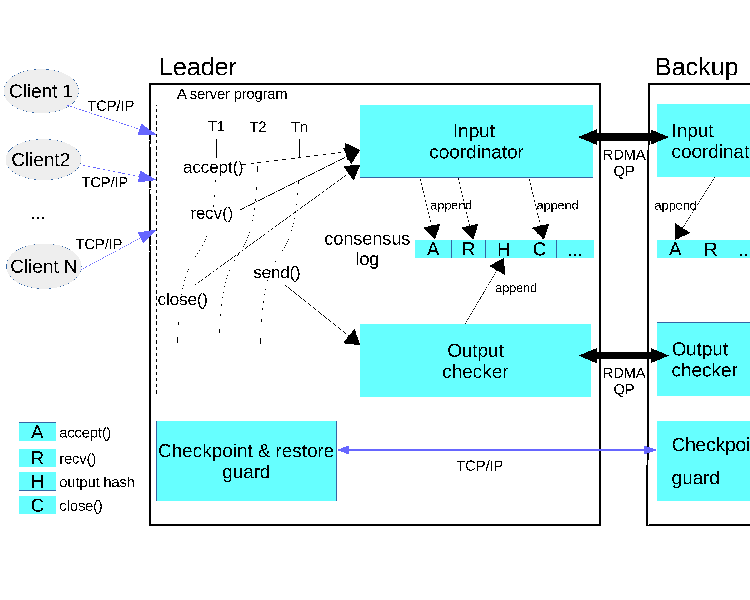
\includegraphics[width=0.31\textheight]{figures/arch.ps}
        \vspace{-.3in}         
        \caption{The \falcon protocol architecture. Protocol components are 
shaded (and in blue color).}
        \label{fig:falcon-arch}
    \end{minipage}
    \centering
    \begin{minipage}{0.48\textwidth}
        \vspace{-.17in}
        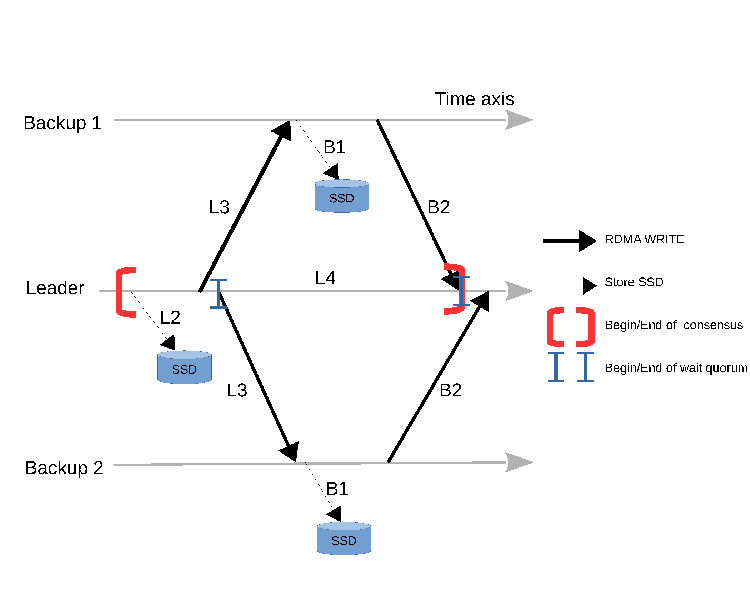
\includegraphics[width=0.34\textheight]{figures/consensus.ps}
        \vspace{-.32in}
        \caption{RDMA-powered consensus algorithm.}
        \label{fig:falcon-protocol}
    \end{minipage}
\end{figure}



With this observation, we propose the design of \falcon,\footnote{Apus is one 
of the fastest birds.} a new RDMA-powered \paxos 
protocol and its runtime system. Figure~\ref{fig:falcon-arch} shows \falcon's 
architecture. It is designed to support unmodified applications. Its runtime 
system will automatically deploy the same application on multiple replicas, 
intercept the application's network inputs from its inbound socket calls (\eg, 
\recv) with a Linux technique called LD\_PRELOAD, and invoke a 
fast, RDMA-powered algorithm (Figure~\ref{fig:falcon-protocol}) to enforce same 
network inputs across replicas. \falcon architecture has four key components: an 
input consensus coordinator and an output checker (both are built on the 
algorithm), an in-memory consensus log, and a guard that handles application 
checkpoints and recovery.

Figure~\ref{fig:falcon-protocol} depicts our algorithm in normal case: the 
leader has four steps (\textbf{L1}$\sim$\textbf{L4}), and each backup has two 
steps (\textbf{B1}$\sim$\textbf{B2}). Leader first executes the actual inbound 
socket call (\textbf{L1}, not shown) to get actual inputs, it then invokes 
consensus across replicas. All solid arrows (\textbf{L3}, \textbf{B2}) are 
one-sided RDMA WRITEs (\S\ref{sec:consensus}) to remote replicas' memory. All 
replicas poll from their own bare memory to receive consensus messages. To 
handle replica failures, all replicas store inputs to local SSD (\textbf{L2}, 
\textbf{B1}). For these WRITEs, sending replicas need only copy data to local 
RDMA NIC and WRITEs return, so \falcon is scalable to replica group size. In 
abnormal cases (\eg, the leader fails), \falcon uses an existing 
algorithm~\cite{paxos:practical} to elect a new leader.

% Three figures. First, falcon arch. Second, consensus protocol. Third, falcon 
% results compared to traditional ones and DARE.



\begin{wrapfigure}{r}{7cm}
  \vspace{-.1in}
  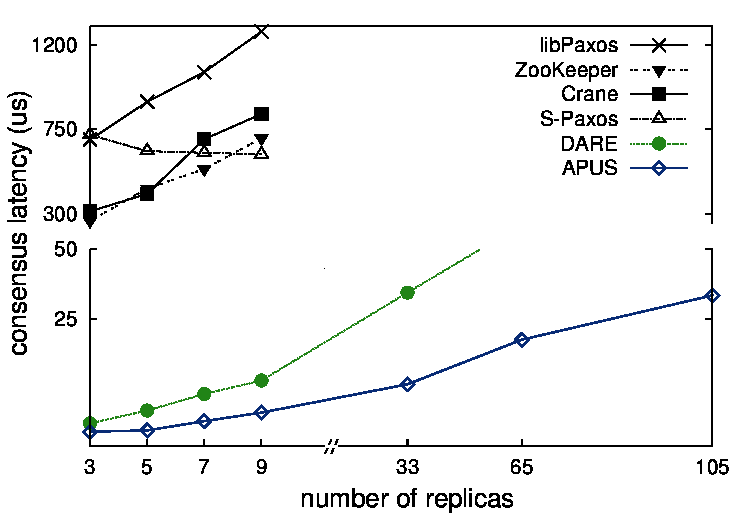
\includegraphics[width=7cm]{figures/traditional_paxos_latency.ps}\\
  \vspace{-.3in}
  \caption{Consensus latency of six \paxos protocols. Both X and Y axes are 
broken to fit in all these protocols. \falcon achieves the smallest consensus 
latency.}
  \label{fig:scalability}
\end{wrapfigure}

% \begin{figure}[!htb]
% \centering
% 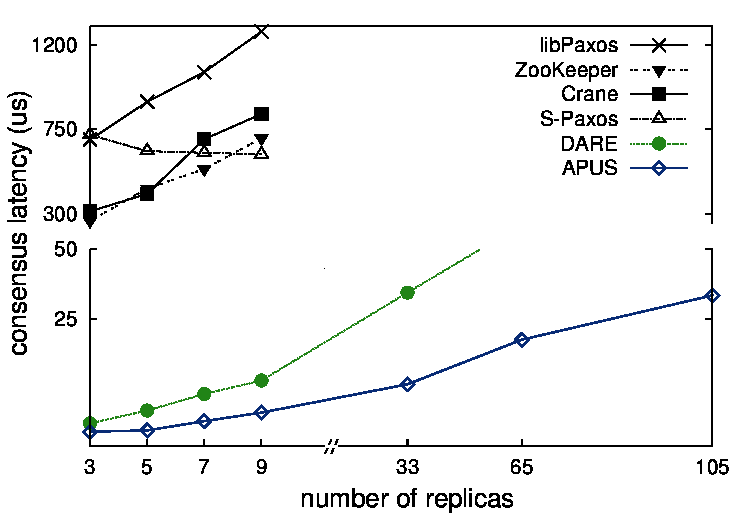
\includegraphics[width=0.25\textheight]{figures/traditional_paxos_latency.ps}
%         \vspace{-.2in}
%         \caption{Consensus latency of six \paxos protocols. \falcon is fastest 
% and scales the best.}
%         \label{fig:scalability}
% \end{figure}

\para{Preliminary results.} We developed an \falcon initial prototype in two 
phases. First, to support unmodified applications, we implemented its 
socket-intercepting runtime system, presented in SOSP 2015~\cite{crane:sosp15}. 
\falcon was able to support 5 widely used server applications (\eg, \mysql) 
without modifying them. Second, recently we implemented its RDMA-powered 
consensus algorithm on a 40Gbps RDMA network. Figure~\ref{fig:scalability} 
shows \falcon performance with 5 existing consensus 
protocols~\cite{crane:sosp15, libpaxos, zookeeper, spaxos:srds12, dare:hpdc15}. 
To analyze the scalability of our algorithm, we ran \falcon and \dare on up to 
105 replicas. \falcon's consensus latency outperforms 4 traditional \paxos  
protocols by \comptradlow to \comptradhigh on 3 to 9 replicas. \falcon is  
faster than \dare by up to \fasterDARE.
% When changing the replica group size 
% from 3 to 105 (a 35x increase), \falcon's consensus latency increases merely 
% from \xxxlatencythree \us to \xxxlatencyonezerofive \us (a \xxxscalability, 
% sub-linear increase).
% Crane. Falcon. Say Crane is first version. Falcon 
% totally subsumes Crane. Falcon also has initial results.



\para{Future work.} We will further improve the practicality of \falcon in two 
dimensions. First, we will extensively evaluate its performance on broad 
latency-critical applications using diverse input workloads. Second, we will 
further torture its scalability on at least 10X more replicas and concurrent 
clients, identify its scalability bottleneck, and refine our algorithm. 

\vspace{-.15in}\subsection{Objective 2: 
building a fault-tolerant scheduler to improve 
application availability}\label{sec:scheduler}\vspace{-.075in}

Many existing schedulers have adopted \paxos to improve availability for 
themselves. Typically, a scheduler use \paxos to replicate its essential 
components such as a \emph{controller}, which handles scheduling computation 
tasks to run on resources. In normal case, only one leading controller does the 
real work, and the other controllers act as backups to in case the leader's 
failure. Unfortunately, most applications run by schedulers have not been 
made highly-available (although individual applications carry a replication 
approach~\cite{mapreduce,dolly:nsdi13}).

A straw-man approach to achieve high application availability could be 
implementing a \paxos protocol for every application. However, this will cause 
two major issues. First, \paxos is notoriously difficult to 
understand~\cite{raft:usenix14,paxos:simple}, implement~\cite{paxos:practical, 
paxos:live}, or test~\cite{modist:nsdi09,demeter:sosp11}. Developing a 
\paxos protocol for every application is widely considered a 
nightmare~\cite{modist:nsdi09,demeter:sosp11,paxos:live} for application 
developers.

The second issue is, schedulers can be conflicting with \paxos due to 
unawareness of an application's \paxos replication scheme. For instance, if an 
application submits multiple replications of the same computation task, a 
scheduler, which abstracts away computer identity, may incorrectly schedule 
some replications on the same computer (it must schedule each replication 
on different computers for \paxos fault-tolerance).

\vspace{-.15in}\subsubsection{\tripod: a first fault-tolerant scheduler 
architecture} 
\label{sec:scheduler-arch}\vspace{-.075in}

% ,\footnote{We name our system after 
% the ancient Chinese three-legged tripod, a reliable, multi-purpose container.}
\tripod replicates all or essential computations of an application. 
It is formed by a widely used scheduler \mesos~\cite{mesos:nsdi11} and 
\falcon (\textbf{Objective 1}). To avoid the two aforementioned issues 
(\S\ref{sec:scheduler}), \tripod's design integrates \paxos in a scheduler, 
not in applications. To achieve high application availability, unlike existing 
schedulers which let only one controller schedule tasks, \tripod runs replicas 
of the same task using replicas of controllers: after controllers agree on a 
new task with \falcon, \tripod lets each controller independently schedule a 
replication of this task. To seamlessly resolve conflicts between the resource 
allocation scheme and replication scheme, \tripod introduces a 
replication-aware 
resource allocation scheme (\S\ref{sec:workflow}).

% Doing so has three benefits. First, \tripod's \paxos acts as a single, general 
% fault-tolerance service to applications. We can just leverage existing 
% verification tools~\cite{modist:nsdi09,demeter:sosp11} to make sure that our 
% \falcon protocol is robust and correct, and then we can benefit many 
% applications. Second, application developers can now just focus on their own 
% application logic, greatly saving development time and money. Third, now 
% \tripod's own scheduler can handle the replication logic and do careful, 
% replication-aware scheduling for jobs  (\S\ref{sec:workflow}). 


% To 
% ahieve application fault-tolerance, 



% In an implementation level, \tripod integrates \mesos~\cite{mesos:nsdi11}, a 
% widely used cluster management system, with a new RDMA-enabled \paxos 
% protocol~\cite{falcon:github}. Compared to a prior RDMA-enabled \paxos 
% protocol~\cite{dare:hpdc15}, our new protocol can support general programs 
% transparently without modifications.

Figure~\ref{fig:scheduler-arch} depicts \tripod's architecture, and its key 
components are shaded (and in blue). To illustrate how \tripod works in an 
application perspective, this figure shows two applications, Hadoop and MPI. 
Each task has a \emph{replica strength} (\vv{R}) to denote the level of 
fault-tolerance it demands. This \vv{R} value is either 1 (default, no 
replication) or no more than the number of controllers in \tripod. An 
application can assign different \vv{R} values to tasks when it submits them 
to \tripod's leader controller.

It is often easy for an application to determine which computation tasks 
are essential and thus require a bigger \vv{R} value. For instance, 
Alluxio~\cite{alluxio}, a distributed storage application ran in \mesos, has 
an essential manager component to manage storages across computers. When 
running in our \tripod scheduler, Alluxio can just assign \vv{R=3} to the 
launching task of its manager.

% By default, each application has \vv{R=1}, which means that this application 
% does not need replication. For such a default setting, \tripod runs the job as 
% is without replication, like a typical cluster management system (\eg, Mesos).

Figure~\ref{fig:scheduler-arch} shows an example of replicating all 
Hadoop~\cite{hadoop} tasks with \vv{R=3}. Suppose Hadoop submits two tasks to 
\tripod's leader controller, each has different shapes (triangle or hexagon). 
The leader controller then invokes a consensus on each task across controllers. 
Once a consensus is reached, each controller assigns the same task on different 
slave computers. The leader controller directly returns its computation result 
to Hadoop. A standby controller ignores computation results until it becomes a 
new leader.
%  unless a tail-tolerance mechanism is triggered 
% (\S\ref{sec:workflow})

% directly save the odp file to eps, level 2.
\vspace{.1in}
\begin{figure}[!htb]
%     \centering
    \begin{minipage}{.48\textwidth}
        \vspace{-.3in}
        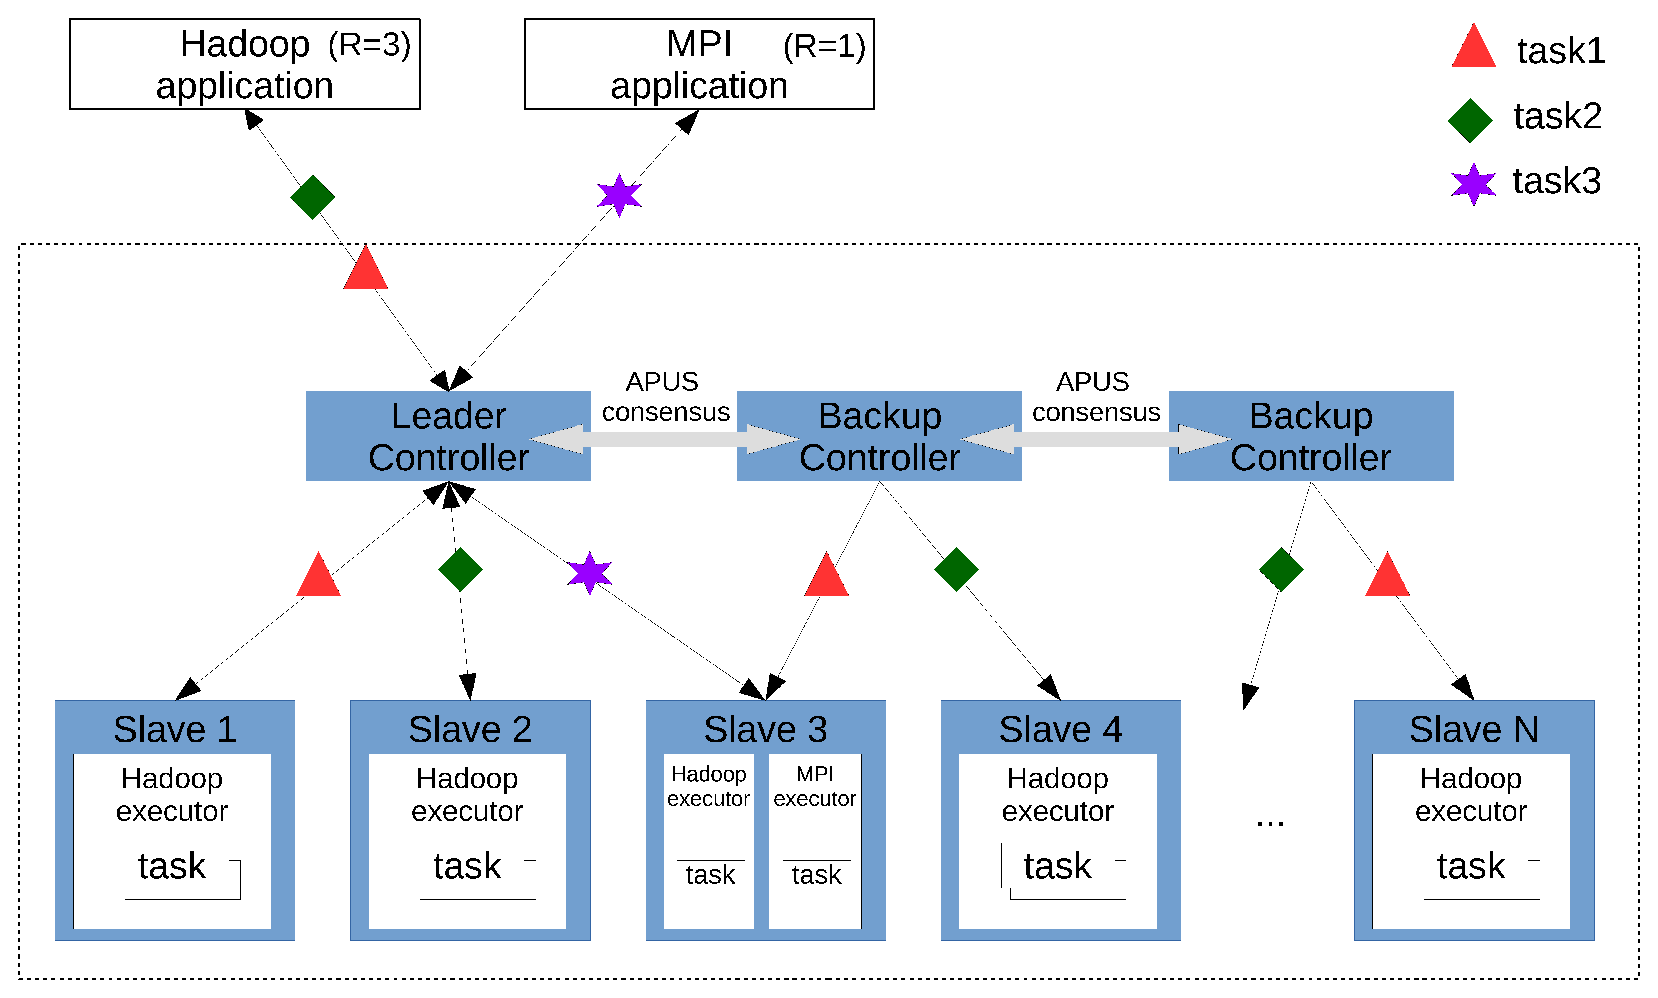
\includegraphics[width=0.34\textheight]{figures/scheduler_arch.eps}
         \vspace{-.4in}
        \caption{\tripod scheduler architecture. It replicates all 
Hadoop~\cite{hadoop} tasks (\vv{R=3}) for fault-tolerance and runs all 
MPI~\cite{mpi} tasks as is (\vv{R=1}).}
        \label{fig:scheduler-arch}
    \end{minipage}
    \hspace{0.16in}
    \begin{minipage}{0.48\textwidth}
        \vspace{-.3in}
        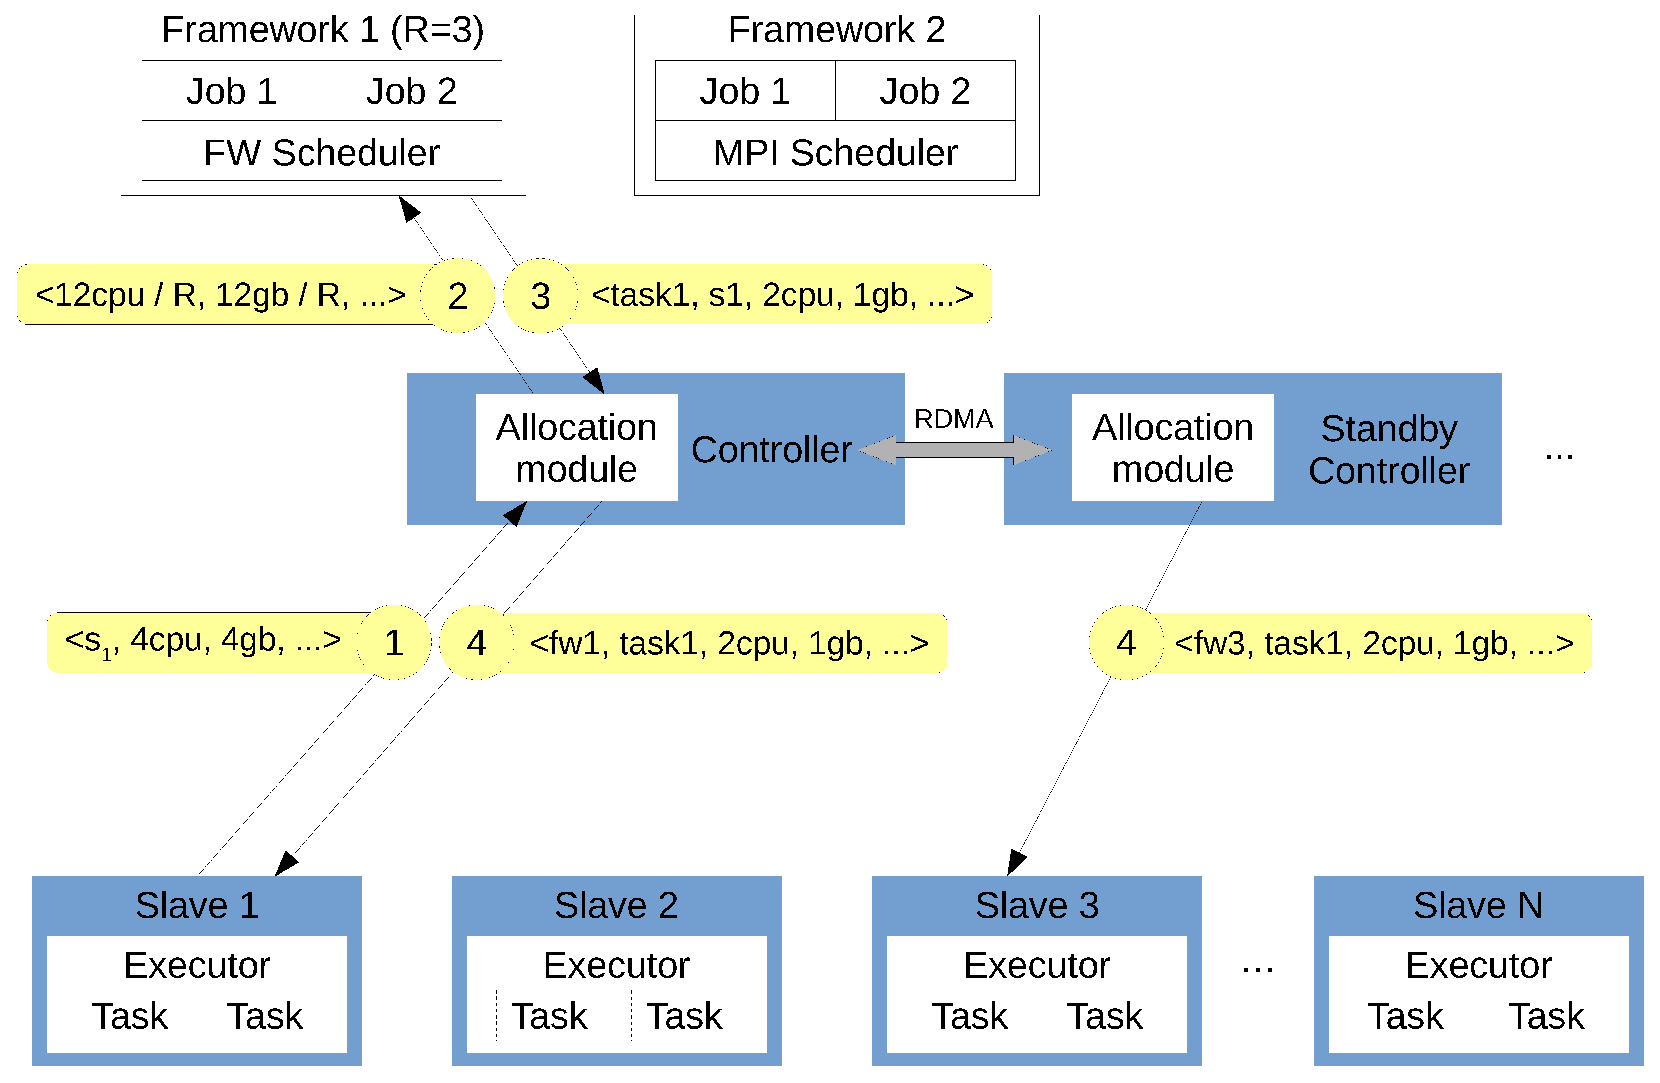
\includegraphics[width=0.34\textheight]{figures/scheduler_flow.eps}
        \vspace{-.4in}
        \caption{The replication-aware resource allocation scheme with four 
steps (\textbf{S1}$\sim$\textbf{S4}).}
        \label{fig:scheduler-workflow}
    \end{minipage}
\end{figure}

% \vspace{-.15in}
\vspace{-.3in}
\subsubsection{Replication-aware resource allocation scheme}
\label{sec:workflow}\vspace{-.075in}

Figure~\ref{fig:scheduler-workflow} shows the design of \tripod's scheme on 
scheduling tasks with four steps. This scheme is similar to that in \mesos 
except the second and fourth steps. In these two steps, \tripod embeds the 
replication logic in its resource offers and allocations for the application. 
An application runs as if \xxx does not replicate any of its tasks, and \tripod 
transparently handles all the replication logic.

In the first step (\textbf{S1}), slave computers periodically report their 
available computing resources (\eg, CPU cores and memory) to the leader 
controller. In the second step (\textbf{S2}), instead of offering the exact 
available resources aggregated from slave computers, \tripod conservatively 
divides the amount of resources by each application's max \vv{R} value and then 
sends a resource offer to the application. The goal is to reserve enough 
resources for \tripod to replicate a task with \vv{R} copies, although some 
tasks have only \vv{R=1}.

In the third step (\textbf{S3}), an application submits tasks with \vv{R} 
values determined by itself to the leader controller. If a task has \vv{R=1}, 
leader schedules the task without consensus and revokes \vv{R-1} resources 
specified in this task from the application. By doing so, the conservatively 
reserved resources are given back to \tripod. If a task has \vv{R>1}, The 
leader then invokes a consensus on this task across controllers.

Once a majority of controllers agrees on executing a task with \vv{R>1}, each 
controller does the fourth step  (\textbf{S4}): it schedules this task on an 
available slave computer according to the resource offer. To prevent 
controllers putting the same task on the same slave computer, the leader 
controller first makes an assignment on which controller should run this task on 
which slave computer, it then carries this assignment in its consensus request. 
Once a consensus on this task is reached, each controller follows this 
assignment.

% Two figures: one is TRIPOD arch. The other is TRIPOD results from the workshop 
% paper. Figure~\ref{fig:scheduler-arch} and Figure~\ref{fig:scheduler-workflow} 
% and Figure~\ref{fig:scheduler-latency}.


% \para{Availability versus resource consumption.} 
\tripod is designed to make a mission-critical application highly available by 
using \vv{R-1} more resources than those consumed by the application's 
essential computations. Non-essential computations use same resources as those 
in \mesos. Given that minor computer failures have caused severe outage 
disasters  (\eg, 2015 NYSE trading halts~\cite{nyse:halt} and several Facebook 
outage events in recent 
years~\cite{facebook:outage}), we consider these extra resource consumptions 
worthwhile on improving application availability.

% We deemed 
% this extra resource consumption reasonable, because even minor computer 
% failures can turn down an entire application. 

% For instance, Both 
% NYSE and Nasdaq have experienced outage of their whole site~\cite{nyse:halt} or 
% specific IPO events~\cite{facebook:ipo:delay} due to minor machine errors. 
% In addition, social-networking applications like Facebook has 
% strong fault-tolerance requirements, because minor machine failures have turned 
% down the whole Facebook site for several times in the last few 
% years~\cite{facebook:outage}, costing huge money lost. 
% for two reasons.
% Second, it is already a common practice to replicate critical computations by 
% using \vv{R} times of resources, and doing so can improve both availability and 
% performance. For instance, Scatter~\cite{scatter:sosp11} runs 8$\sim$12 
% replicas in a \paxos group to order client requests, and it lets replicas reply 
% requests in parallel. A bigger group size will improve Scatter throughput. 
% Moreover, several recent replication 
% systems~\cite{eve:osdi12,rex:eurosys14,crane:sosp15} 
% improve the availability of general server applications (\eg, 
% \mysql~\cite{mysql}) by replicating them.

% Therefore, \tripod's design favors more on availability and performance 
% (low consensus latency). It's design tends to use \vv{R} times of resources 
% compared to traditional applications. We argue that this extra resource 
% utilizations are acceptable for critical applications, because if they have 
% high 
% demand on availability and response times, they can often tolerate costs on 
% computing resources (\eg, trading and medical platforms).



\para{Preliminary results.} We presented an early prototype of \tripod
in APSys 2016~\cite{tripod:apsys16}. To evaluate a typical social-networking 
application, we ran \tripod with \redis~\cite{redis}, a key-value store used by 
Twitter and financial platforms~\cite{nosql:finance}. Although \redis is a 
latency-critical application, compared to its own unreplicated execution, 
\tripod incurred merely \tputoverhead overhead in throughput and 
\latencyoverhead in response time.
% This protocol was 40.1X faster than \zookeeper, a traditional replication
% protocol~\cite{calvin:sigmod12} which runs on TCP/IP.

% Disable the figure for now. Not much information.
% \begin{figure}[!htb]
% \centering
% 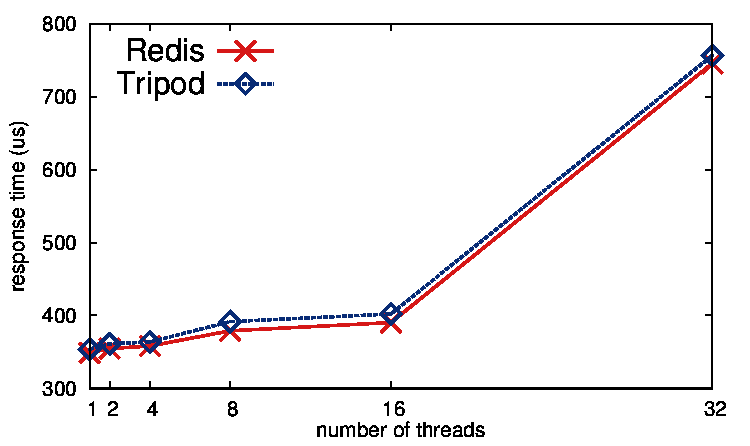
\includegraphics[width=0.34\textheight]{figures/scheduler_latency.ps}
%         \vspace{0.1in}
%         \caption{Performance overhead of scheduler.}
%         \label{fig:scheduler-latency}
% \end{figure}

\para{Future directions.} We foresee three directions for \tripod's future 
development. First, we will further improve the performance of its 
replication-aware resource allocation scheme through an extensive study on 
diverse applications. Second, currently this scheme is tied to \mesos. We will 
study other popular schedulers, summarize general resource allocation scheme 
patterns, then we will develop a scheduler-agnostic scheme for general 
datacenter schedulers. Third, currently this scheme requires application 
developers to determine \vv{R} values for application components. We will 
leverage our expertise on precise 
program analysis~\cite{peregrine:sosp11,woodpecker:asplos13} to create new 
schemes that can automatically analyze an application and assign precise \vv{R} 
values to different components. We believe that all these directions will 
generate new conceptual methods.

\vspace{-.15in}\subsection{Objective 3: building a new fault-tolerant VM 
replication architecture}\label{sec:vm}\vspace{-.075in}

%% TBD: must emphasis that primary-backup or migration will clean up dirty 
% % pages after the transfer, otherwise the tree will become bigger and bigger 
% and we have not optimization.

% Virtual machines (VM) infrastructures (\eg, Amazon EC2~\cite{amazon:vpc} and 
% OpenStack~\cite{openstack}) are widely deployed in datacenters and clouds 
% because they can provide a virtualized abstraction of computing resources to 
% different applications and enforce strong utilization isolation and security. 

Existing VM fault-tolerance architectures are based on two similar 
techniques: primary-backup and live migration (\S\ref{sec:others-work}). For 
instance, after processing every request, the primary-backup technique 
transfers all memory pages modified by applications (\ie, dirty pages in 4KB) 
from the primary to backup. This technique consumes 2*\vv{V} resources (\vv{V} 
denotes resource volumn consumed by an unreplicated execution). Although 
these two techniques are adopted by industry~\cite{ftvm,vmotion:atc05}, a major 
problem is that the transfered dirty bytes can be up to 1.7GB 
(\S\ref{sec:tracking}), causing a substantial  delay and network bandwidth 
consumption for \emph{every} request.

A key reason for this problem is that existing techniques have only one real 
application execution. We will use \falcon (\textbf{Objective 1}) to tackle 
this problem as it maintains multiple real executions. By using \falcon to 
enforce same inputs across VM replicas, most dirty pages across replicas are 
same and needn't transfer.

% , these two 
% existing techniques 
% face the problems of significant application downtime (\eg, 8 seconds in 
% vMotion~\cite{vmotion:atc05}) and network bandwidth consumption.

%  Therefore, to transfer dirty pages to a 
% remote computer, substantial downtime and network bandwidth consumption are 
% unavoidable.




% Therefore
% Mainly introduce EC2, Openstak. VM only.

% Briefly introduce VM fault-tolerance techniques. Primary-backup. Remus. 
% Hypervisor replication (old paper). FaRM.
% 
% Talk about migration. It is similar to primary-backup, but mainly for load 
% balance, not to overcome failures. Main approach is live migration that aims to 
% reduce application down time. VMotion.

% However, there is still substantial down time and resource consumption. E.g., 
% vMotion, for memory intensive applications, the down time can be up to 30 
% seconds. As migration tends to invoke frequently for load balancing, 
% consolidation, energy saving, this downtime may incur big money lost for cloud 
% deployers.

% When doing migration, both the local computer and the migration destination 
% computer incur big resource consumption. This is contraditive to the motivation 
% of migration: reduing computer loads on the local computer.

\vspace{-.15in}\subsubsection{Integrating \falcon into the KVM hypervisor 
layer} 
\label{sec:vm-arch}\vspace{-.075in}

% \begin{figure}[!htb]
% \centering
% \vspace{-.2in}
% 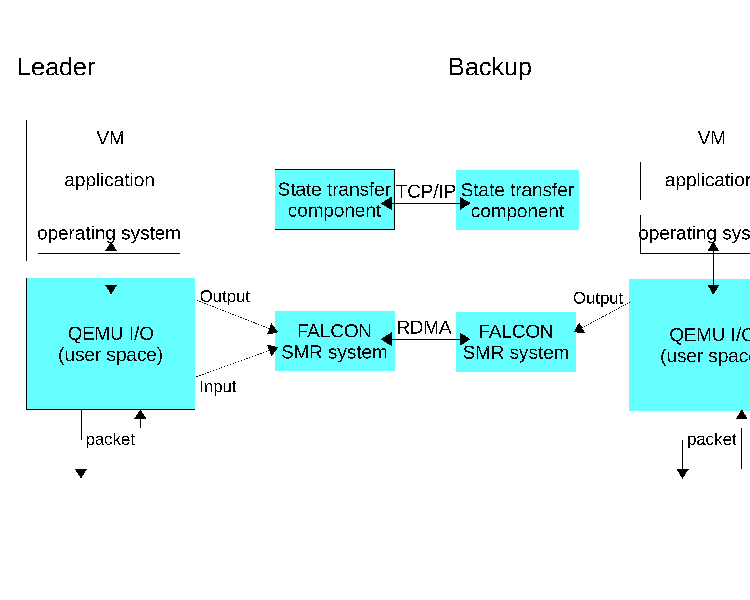
\includegraphics[width=0.25\textheight]{figures/vm_arch.ps}
%         \vspace{-.3in}
%         \caption{The \falcon and KVM eco-system.}
%         \label{fig:vm-arch}
%         \vspace{-.2in}
% \end{figure}








% We will inte \falcon 
% into the hypervisor layer of popular VMs. 
We choose KVM~\cite{kvm} as our base VM for two main reasons. First, KVM 
is a mature, open source hypervisor in Linux. Second, it provides 
\vv{tap\_send()}, an input capturing API in its hypervisor. This API allows 
\falcon to intercept network inputs on the leader VM and transparently 
replicates them on backup VMs.
% Third, this KVM API runs in 
% user-space, which allows RDMA to work (RDMA runs in user-space).

%% Consume same resources as primary-backup.
We proactively design our VM replication architecture to maintain same 2*\vv{V} 
resource consumption as existing VM fault-tolerance techniques. Although \paxos 
consumes 3*\vv{V} resources, our design reduces \vv{V} resources by letting 
one backup act as the \emph{major backup} with a high priority to become a new 
leader if current leader fails. The major backup agrees on and executes input 
requests, and the other backup acts as the \emph{standby backup} which only 
agrees on requests without executing them (\ie, without consuming \vv{V} 
resources). In total, 2*\vv{V} resources are consumed by the leader and major 
backup in our VM. To maintain the same fault-tolerance guarantee as \paxos (\ie, 
to in case the standby backup being elected a leader), the major backup 
periodically does a standard checkpoint operation as in existing 
works~\cite{crane:sosp15,rex:eurosys14} and sends it to the standby backup. 
Although a checkpoint operation will slow down the major backup, it does not 
affect our performance because the leader and standby backup still form a 
majority and agree on requests rapidly.
% Therefore, even if the standby backup is elected a new leader, it extracts 
% checkpoints and uses the agreed inputs to catch up with old leader quickly.

% If the leader 
% fails, \falcon gives the major backup a high priority to become the new leader.

% This design has three important benefits: (1) our new VM fault-tolerance 
% technique consumes roughly same 2*\vv{R} computing resources as existing 
% techniques; (2) a \paxos majority group still holds; (3) it is robust 
% because even if the standby backup is elected as a new leader, it can extract 
% checkpoints and use the aggreed inputs to catch up with the old leader quickly.

% Figure~\ref{fig:vm-arch} shows the architecture of the eco-system. To provide 
% the same fault-tolerance guarantee with primary-backup, a typical replication 
% factor of this eco-system is \vv{R=3}. 

% A key benefit of such a \paxos-based VM replication over primary-backup is that 
% its leadership is strongly consistent (through a majority agreement, which 
% primary-backup lacks), and it saves the bandwidth consumption for transferring 
% application execution states in primary-backup.

\vspace{-.15in}\subsubsection{A new synchronization technique to 
track divergent pages across VM replicas}
\label{sec:tracking}\vspace{-.075in}



Although our VM architecture enforces same inputs across VM replicas, 
minor memory pages may still diverge across replicas (\eg, due to 
data races~\cite{lu:concurrency-bugs}). We propose a synchronization 
technique to efficiently track and transfer divergent pages, including (1) 
an efficient \vv{O(log N)} algorithm to track divergent pages, and (2) 
leveraging \falcon's RDMA-powered protocol to efficiently and reliably compare 
divergent pages.

A naive way is linearly comparing all \vv{N} dirty pages between replicas to 
find divergent ones, but it is as slow as prior primary-backup 
techniques. Instead, our algorithm uses a Merkle tree~\cite{eve:osdi12} to track 
dirty pages on each replica. As shown in Figure~\ref{fig:vm-tree}, if a 
physical page is modified, our VM hypervisor appends it as a leaf to a
Merkle and incrementally recomputes a  hash with the page content towards all 
parents. This tree is efficient because if the roots of two trees 
have same hash, all leaves (pages) are the same.

% Three steps.
However, our VM architecture poses a new interesting challenge: unlike 
previous works that tree leaves are static (\eg, Eve~\cite{eve:osdi12} treats 
static global variables in application code as leaves), the leaves in our trees 
are dynamic as they are dirty pages. Because dirty pages across replicas can be 
different, the structures (\ie, the number of internal nodes) of Merkle trees 
between two replicas can be different and hard to compare.

Our synchronization technique tackles this challenge by introducing a 
\emph{tree adjustment} phase. It works with four steps. First, after 
processing one request, leader sends a dirty page bitmap provided by KVM to 
the major backup. Major backup does a union on this bitmap and its own one 
and sends back to leader. Second, both leader and the major backup do 
a tree adjustment with the union bitmap (\eg, a non-dirty page in the union is 
still appended to the tree), then leader and the backup's trees have same leaves 
and same structure. Third, leader invokes \textbf{Algorithm 1} to do a 
\vv{O(log N)} traversal from tree root to find divergent leaves. To compare 
internal node hashes between leader and backup, the algorithm invokes an 
augmented \falcon protocol as \textbf{APUS()}, which returns divergent nodes 
carried in the backup's consensus reply. Fourth, leader transfers divergent 
pages to the major backup, then they both clear trees and dirty page flags.

% directly save the odp file to eps, level 2.
\begin{figure}[!htb]
%     \begin{minipage}{.49\textwidth}
%         \vspace{-.2in}
%         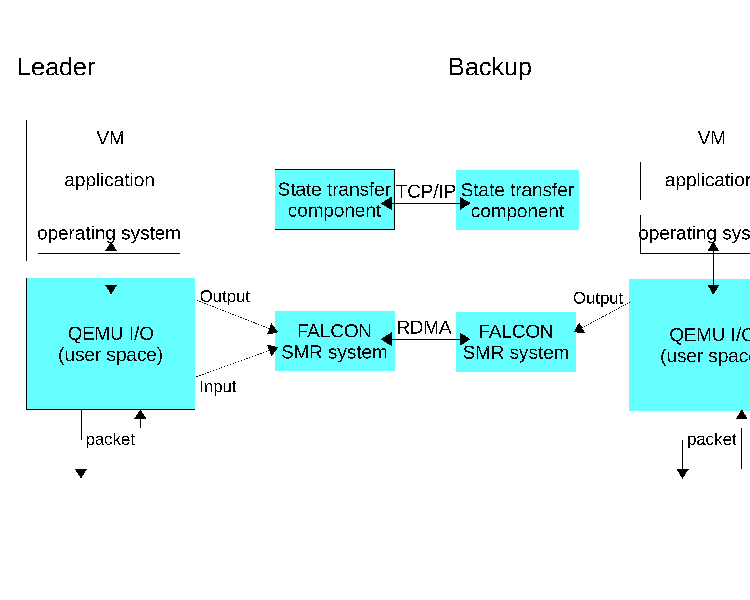
\includegraphics[width=0.34\textheight]{figures/vm_arch.ps}
%         \vspace{-.3in}
%         \caption{A new fault-tolerant VM for improving application 
% availability.}
%         \label{fig:vm-arch}
%     \end{minipage}
    \begin{minipage}{0.47\textwidth}
        \vspace{-.2in}
        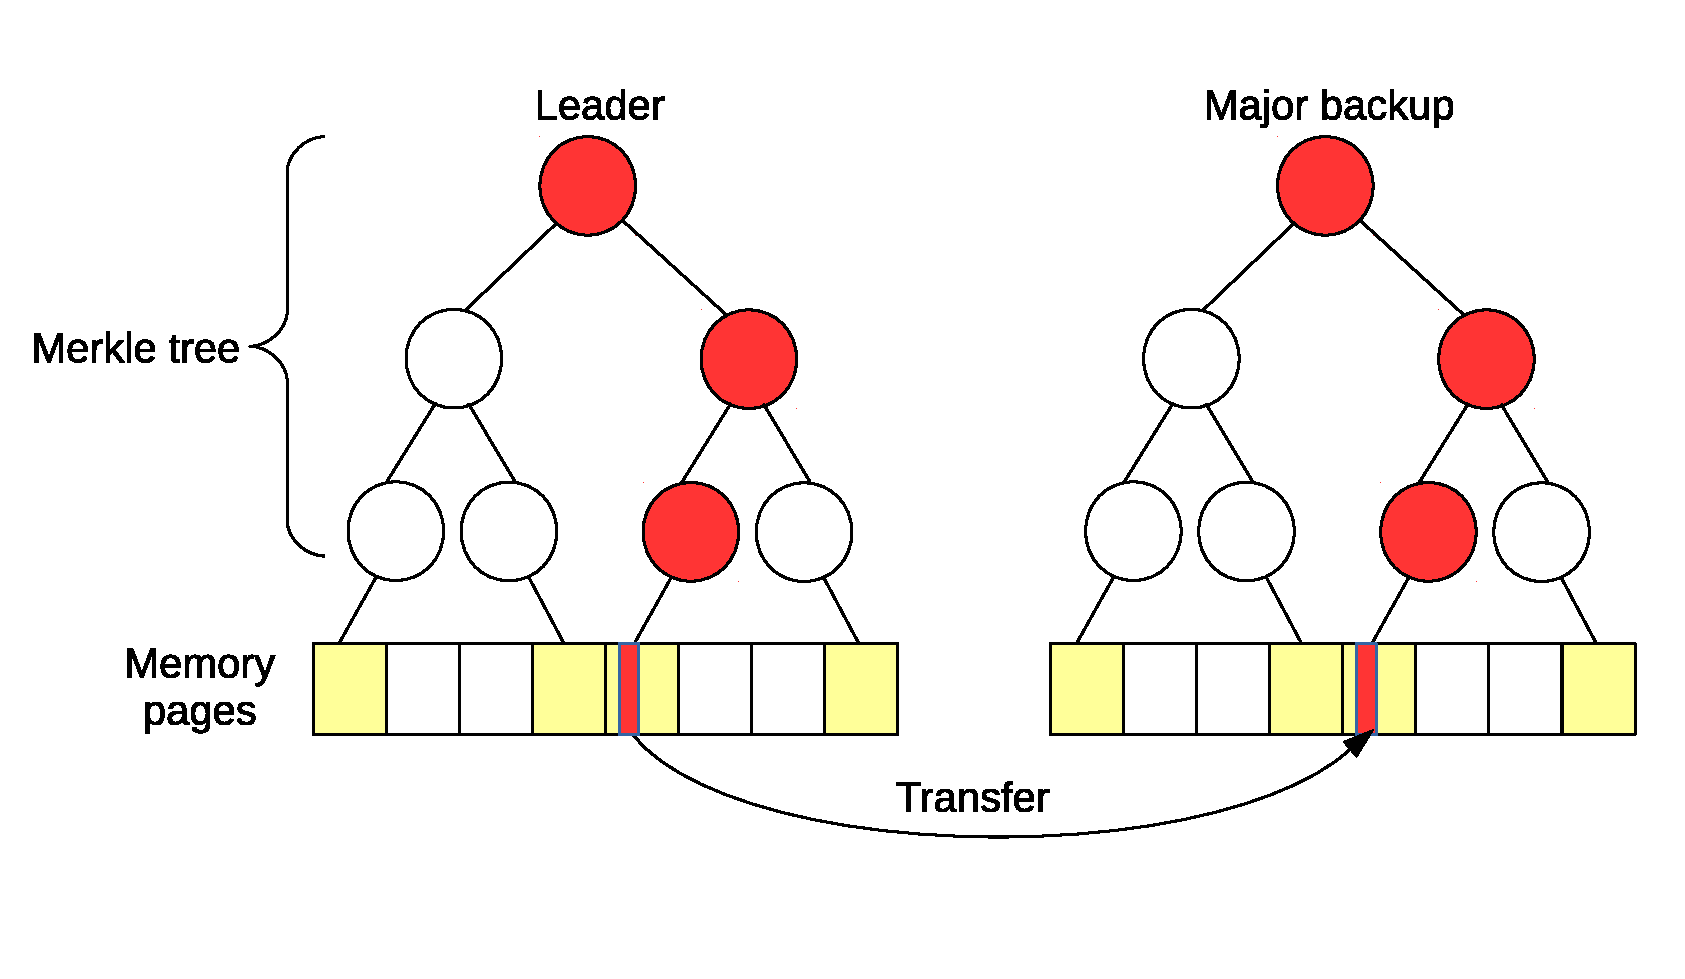
\includegraphics[width=0.33\textheight]{figures/tree.eps}
        \vspace{-.3in}
        \caption{Data structures on tracking divergent dirty pages across 
replicas. Dirty pages are in yellow; divergent dirty pages and parents 
are in red.}
        \label{fig:vm-tree}
    \end{minipage}
    \begin{minipage}{0.52\textwidth}
      \vspace{-.2in}
      \centering
      \begin{algorithm}[H]
      \DontPrintSemicolon
      \scriptsize
      \SetCommentSty{textrm}
      \SetKwInOut{Input}{Input}
      \SetKwInOut{Output}{Output}
      \Input{The root of Merkle tree on leader, $root$}
      \Output{Different memory pages between leader and replica, $pages$}
      
      \SetKwBlock{Titlea}{Track($root$)}{end}
      \Titlea {
%         $diverged$ $\leftarrow$ empty sequence \;
        $pages$ $\leftarrow$ empty sequence \;
        $diverged$ $\leftarrow$ \textbf{APUS}($root$, $root$.left(), 
$root$.right()) \;
        \For {{\rm $i$ $\leftarrow$ $diverged$.push\_front()}} {
          \If {{\rm $i$ is\_leaf()}} {
            $pages$.append($i$) \;
          }
          \Else {
            $diff$ $\leftarrow$ \textbf{APUS}($i$, $i$.left(), 
$i$.right()) \;
            $diverged$.append($diff$) \;
          }
        }
        \Return $pages$ \;
      }
      \caption{Tracking divergent memory pages}
      \label{alg:slice}
      \end{algorithm}
    \vspace{-.1in}
    %     \caption{Sketch of path slicing algorithm}

%         \label{fig:algo}

\end{minipage}
    \vspace{-.1in}
\end{figure}

To see whether divergent pages are indeed rare, we ran three applications, 
MongoDB~\cite{mongodb}, Redis~\cite{redis}, and Memcached~\cite{memcached}, on 
two KVMs with same real-world workloads~\cite{ycsb}. We 
found 261.1K$\sim$429K dirty pages (\ie, up to 1.7GB). Primary-backup 
techniques have to transfer all dirty pages. We also found that only 
14.2$\sim$29.3K of these dirty pages diverged between two VMs. These initial 
results imply that \textbf{Algorithm 1} can reduce up to 96.7\% transfered pages 
compared to primary-backup techniques.

% To do this, each replica 
% maintains a Merkle tree kept 
% updating from the dirty pages. By "dirty", we mean the memory page has been 
% modified since last synchronization. One problem here is that each VM may have 
% dirtied different pages. This leads to different structures of Merkle trees and 
% they are not comparable. \xxx addresses this problem using a fast method as 
% follows:

% \begin{small} \textit{(We use $A$ to denote the diverged replica; it will fetch 
% state 
% from replica $B$)} \end{small}
% \begin{enumerate}
% \item $A$ sends its dirty page bitmap $M_A$ to $B$.
% \item $B$ does a \textit{bitwise or} calculation \ $M_{union} = M_A | M_B $, 
% and sends $M_{union}$ back to $A$.
% \item $A$ and $B$ both update their own Merkle tree according to $M_{union}$. 
% $A$ sends its updated Merkle tree to $B$. 
% \item $B$ does a comparison on both Merkle tress to find the differences, as 
% illustrated in Figure~\ref{fig:tree}.
% \end{enumerate}

% Our method is efficient for two reasons. First, it only transfers the different 
% pages between replicas. Because we have made consensus on inputs and we can 
% turn off \textit{Address Space Layout Randomization} to trade for correctness, 
% the difference rate will be really small. Second, the use of Merkle tree 
% optimizes the time complexity of comparison between memory states to $O(\log 
% n)$.

% Describe the infrastructure. Take Ning's figure. Hypervisor. tap\_send().

% \vspace{-.15in}\subsubsection{\paxos-based Live Migration} 
% \label{sec:vm-migration}\vspace{-.075in}
% 
% Interestingly, this replication ability not only provides high 
% availability for fault-tolerance (suitable for the primary-backup scenario), 
% but can also greatly save resource consumption if fault-tolerance is not a 
% major concern (suitable for the live migration scenario). Consider the live 
% migration scenario, \paxos backups can only agree on inputs without actually 
% executing them, then the overall application execution consumes almost same 
% resources as the unreplicated one. A backup now can just absorb occasional, 
% periodical application checkpoints from the leader when the leader replica is 
% idle, and catches up with the leader when a migration destination is decided on 
% this backup.
% 
% % We propose our own replication approach. The non-leader only agree on new 
% % inputs, they can opt to execute requests or absorb periodic checkpoints.
% Leveraging this idea, we propose a fast, network bandwidth-friendly live 
% migration approach called ``\paxos-based live migration". A key benefit of this 
% approach is that, now migration does not require transferring all execution 
% states of application, but only transferring the \paxos leadership (almost as 
% fast as \paxos consensus latency) to a destination backup which has idle 
% resources. To increase the chance on finding a proper destination, we can 
% leverage \falcon's high availability to run many backups within a datacenter.

% This approach is othorgnal to the VM replication. 
% This \paxos-based live migration approach contains four steps. First, in 
% normal case, the current computing instance (the leader) just agrees on 
% incoming inputs with backups using \falcon. A set of backups run on highly 
% loaded computers and agree on inputs (also record the inputs persistently). 
% 
% Second, the leader does a periodical checkpoint when it's idle (no incoming 
% requests), and sends the checkpoint to the backups. The backups only keeps 
% the latest checkpoint and discards prior ones.
% 
% Third, when the VM invokes a migration on the leader computer, it uses a 
% standard migration mechanism to determine which backup should be the migration 
% destination (the next leader). Then, the destination extracts the latest
% checkpoint on local computer, restores the application state, and then catches 
% up with the leader with executing the recorded but not executed inputs.
% 
% Fourth, we invoke a \falcon protocol level operation: migration the 
% leadership, which is similar to a traditional \paxos leader election 
% process~\cite{paxos:practical}, but we just explicitly decide the destination 
% computer as the new leader. \falcon's protocol handles various failure 
% scenarios (\eg, the destination computer crashes during the migration) as its 
% \paxos nature.

% TBD: mention the leader election latency in Objective 2.
% Analysis: this approach incurs almost zero time and resource for a few reasons. 
% First, the leadership migration is fast (tens of micro seconds). Second, no 
% frequent execution state transfer during the migration time, only at the 
% leader's idle time. Third, robust to various scenarios (\eg, destination fails 
% during the migration), thanking to \paxos.

\para{Future directions.} We anticipate broad research outcomes in two 
directions. First, we will implement our algorithm and quantify its performance 
improvement compared to existing primary-backup techniques (\eg, 
vSphere~\cite{ftvm}). Second, we will apply the algorithm to develop new 
lightweight VM live migration techniques (\S\ref{sec:others-work}). Because VM 
primary-backup and migration techniques are applied to address broad challenges 
(\eg, improving resource utilization, balancing computer loads, and saving 
datacenter energy), applications of our techniques on these challenges will 
cultivate even broader innovative techniques.


% % TBD: need a new replication approach name.
% \vspace{-.15in}\subsubsection{Idea I: Hybrid Replication} 
% \label{sec:defense-arch}\vspace{-.075in}
% 
% TBD.

\vspace{-.15in}\subsection{Research plan} \label{sec:plan}\vspace{-.075in}

This project will require two PhD students S1 and S2 to work for 
three years. In the first year, S1 will design and fully implement the \falcon 
protocol (part of \textbf{Objective~1}), and S2 will evaluate its performance 
and robustness on various real-world storage applications (part of 
\textbf{Objective~1}). In the second year, S1 will 
integrate \falcon to a scheduler \mesos (part of \textbf{Objective~2}), and S2 
will make \falcon and KVM form an eco-system (part of \textbf{Objective~3}). In 
the third year, S1 and S2 will respectively evaluate the efficacy of their 
infrastructures built from \textbf{Objective 2} and \textbf{Objective 3} on 
diverse
real-world applications.
% Both students will 
% involve theoretical methods, implement real software systems, and 
% perform real-world study.
% The PI will supervise the students by providing 
% advice concerning both theoretical and systems implementation levels.


